
%%%%%%%%%%%%%%%%%%%%%%%%%%%%%%%%%%%%%%%%%
% Programming/Coding Assignment
% LaTeX Template
%
% This template has been downloaded from:
% http://www.latextemplates.com
%
% Original author:
% Ted Pavlic (http://www.tedpavlic.com)
%
% Note:
% The \lipsum[#] commands throughout this template generate dummy text
% to fill the template out. These commands should all be removed when 
% writing assignment content.
%
% This template uses a Perl script as an example snippet of code, most other
% languages are also usable. Configure them in the "CODE INCLUSION 
% CONFIGURATION" section.
%
%%%%%%%%%%%%%%%%%%%%%%%%%%%%%%%%%%%%%%%%%

%----------------------------------------------------------------------------------------
%	PACKAGES AND OTHER DOCUMENT CONFIGURATIONS
%----------------------------------------------------------------------------------------



\documentclass{article}

\usepackage{fancyhdr} % Required for custom headers
\usepackage{lastpage} % Required to determine the last page for the footer
\usepackage{extramarks} % Required for headers and footers
\usepackage[usenames,dvipsnames]{color} % Required for custom colors
\usepackage{graphicx} % Required to insert images
\usepackage{listings} % Required for insertion of code
\usepackage{courier} % Required for the courier font
\usepackage{lipsum} % Used for inserting dummy 'Lorem ipsum' text into the template
\usepackage{setspace}
\usepackage{color}
\usepackage{comment}
\usepackage{caption}
\usepackage[T1]{fontenc}
\usepackage{hyperref}
\usepackage{natbib}
\usepackage{underscore}
\usepackage{subfigure}
\usepackage{fixltx2e}

\hypersetup{
    colorlinks=true,
    linkcolor=blue,
    filecolor=magenta,      
    urlcolor=cyan,
    breaklinks=true
}

\usepackage[]{algorithm2e}
\usepackage{pdfpages}
\usepackage{tikz}




%For python inclusion (http://widerin.org/blog/syntax-highlighting-for-python-scripts-in-latex-documents)
\definecolor{Code}{rgb}{0,0,0}
\definecolor{Decorators}{rgb}{0.5,0.5,0.5}
\definecolor{Numbers}{rgb}{0.5,0,0}
\definecolor{MatchingBrackets}{rgb}{0.25,0.5,0.5}
\definecolor{Keywords}{rgb}{0,0,1}
\definecolor{self}{rgb}{0,0,0}
\definecolor{Strings}{rgb}{0,0.63,0}
\definecolor{Comments}{rgb}{0,0.63,1}
\definecolor{Backquotes}{rgb}{0,0,0}
\definecolor{Classname}{rgb}{0,0,0}
\definecolor{FunctionName}{rgb}{0,0,0}
\definecolor{Operators}{rgb}{0,0,0}
\definecolor{Background}{rgb}{0.98,0.98,0.98}

% Margins
\topmargin=-0.45in
\evensidemargin=0in
\oddsidemargin=0in
\textwidth=6.5in
\textheight=9.0in
\headsep=0.25in

\linespread{1.1} % Line spacing

% Set up the header and footer
\pagestyle{fancy}
\lhead{\hmwkAuthorName} % Top left header
\chead{\hmwkClass\ (\hmwkClassInstructor\ \hmwkClassTime): \hmwkTitle} % Top center head
\chead{\hmwkClass\ (\hmwkClassInstructor): \hmwkTitle} % Top center head
\rhead{\firstxmark} % Top right header
\lfoot{\lastxmark} % Bottom left footer
\cfoot{} % Bottom center footer
\rfoot{Page\ \thepage\ of\ \protect\pageref{LastPage}} % Bottom right footer
\renewcommand\headrulewidth{0.4pt} % Size of the header rule
\renewcommand\footrulewidth{0.4pt} % Size of the footer rule

\setlength\parindent{0pt} % Removes all indentation from paragraphs

%----------------------------------------------------------------------------------------
%	CODE INCLUSION CONFIGURATION
%----------------------------------------------------------------------------------------

\definecolor{MyDarkGreen}{rgb}{0.0,0.4,0.0} % This is the color used for comments
\lstloadlanguages{Perl} % Load Perl syntax for listings, for a list of other languages supported see: ftp://ftp.tex.ac.uk/tex-archive/macros/latex/contrib/listings/listings.pdf
\lstset{language=Perl, % Use Perl in this example
        frame=single, % Single frame around code
        basicstyle=\small\ttfamily, % Use small true type font
        keywordstyle=[1]\color{Blue}\bf, % Perl functions bold and blue
        keywordstyle=[2]\color{Purple}, % Perl function arguments purple
        keywordstyle=[3]\color{Blue}\underbar, % Custom functions underlined and blue
        identifierstyle=, % Nothing special about identifiers                                         
        commentstyle=\usefont{T1}{pcr}{m}{sl}\color{MyDarkGreen}\small, % Comments small dark green courier font
        stringstyle=\color{Purple}, % Strings are purple
        showstringspaces=false, % Don't put marks in string spaces
        tabsize=5, % 5 spaces per tab
        %
        % Put standard Perl functions not included in the default language here
        morekeywords={rand},
        %
        % Put Perl function parameters here
        morekeywords=[2]{on, off, interp},
        %
        % Put user defined functions here
        morekeywords=[3]{test},
       	%
        morecomment=[l][\color{Blue}]{...}, % Line continuation (...) like blue comment
        numbers=left, % Line numbers on left
        firstnumber=1, % Line numbers start with line 1
        numberstyle=\tiny\color{Blue}, % Line numbers are blue and small
        stepnumber=5 % Line numbers go in steps of 5
}

% Creates a new command to include a perl script, the first parameter is the filename of the script (without .pl), the second parameter is the caption
\newcommand{\perlscript}[2]{
\begin{itemize}
\item[]\lstinputlisting[caption=#2,label=#1]{#1.pl}
\end{itemize}
}


%----------------------------------------------------------------------------------------
%	DOCUMENT STRUCTURE COMMANDS
%	Skip this unless you know what you're doing
%----------------------------------------------------------------------------------------

% Header and footer for when a page split occurs within a problem environment
\newcommand{\enterProblemHeader}[1]{
\nobreak\extramarks{#1}{#1 continued on next page\ldots}\nobreak
\nobreak\extramarks{#1 (continued)}{#1 continued on next page\ldots}\nobreak
}

% Header and footer for when a page split occurs between problem environments
\newcommand{\exitProblemHeader}[1]{
\nobreak\extramarks{#1 (continued)}{#1 continued on next page\ldots}\nobreak
\nobreak\extramarks{#1}{}\nobreak
}

\setcounter{secnumdepth}{0} % Removes default section numbers
\newcounter{homeworkProblemCounter} % Creates a counter to keep track of the number of problems

\newcommand{\homeworkProblemName}{}
\newenvironment{homeworkProblem}[1][Problem \arabic{homeworkProblemCounter}]{ % Makes a new environment called homeworkProblem which takes 1 argument (custom name) but the default is "Problem #"
\stepcounter{homeworkProblemCounter} % Increase counter for number of problems
\renewcommand{\homeworkProblemName}{#1} % Assign \homeworkProblemName the name of the problem
\section{\homeworkProblemName} % Make a section in the document with the custom problem count
\enterProblemHeader{\homeworkProblemName} % Header and footer within the environment
}{
\exitProblemHeader{\homeworkProblemName} % Header and footer after the environment
}

\newcommand{\problemAnswer}[1]{ % Defines the problem answer command with the content as the only argument
\noindent\framebox[\columnwidth][c]{\begin{minipage}{0.98\columnwidth}#1\end{minipage}} % Makes the box around the problem answer and puts the content inside
}

\newcommand{\homeworkSectionName}{}
\newenvironment{homeworkSection}[1]{ % New environment for sections within homework problems, takes 1 argument - the name of the section
\renewcommand{\homeworkSectionName}{#1} % Assign \homeworkSectionName to the name of the section from the environment argument
\subsection{\homeworkSectionName} % Make a subsection with the custom name of the subsection
\enterProblemHeader{\homeworkProblemName\ [\homeworkSectionName]} % Header and footer within the environment
}{
\enterProblemHeader{\homeworkProblemName} % Header and footer after the environment
}

%----------------------------------------------------------------------------------------
%	NAME AND CLASS SECTION
%----------------------------------------------------------------------------------------

\newcommand{\hmwkTitle}{Assignment\ \#3 } % Assignment title
%\newcommand{\hmwkDueDate}{Monday,\ January\ 1,\ 2012} % Due date
\newcommand{\hmwkClass}{Web Science} % Course/class
%\newcommand{\hmwkClassTime}{10:30am} % Class/lecture time
\newcommand{\hmwkClassInstructor}{Alexander Nwala} % Teacher/lecturer
\newcommand{\hmwkAuthorName}{Puneeth Bikkasandra} % Your name

%----------------------------------------------------------------------------------------
%	TITLE PAGE
%----------------------------------------------------------------------------------------

\title{
\vspace{2in}
\textmd{\textbf{\hmwkClass:\ \hmwkTitle}}\\
%\normalsize\vspace{0.1in}\small{Due\ on\ \hmwkDueDate}\\
%\vspace{0.1in}\large{\textit{\hmwkClassInstructor\ \hmwkClassTime}}
\vspace{0.1in}\large{\textit{\hmwkClassInstructor}}
\vspace{3in}
}

\author{\textbf{\hmwkAuthorName}}
\date{Wednesday, February 21, 2018} % Insert date here if you want it to appear below your name

%----------------------------------------------------------------------------------------

\begin{document}

\maketitle
\newpage



%----------------------------------------------------------------------------------------
%	TABLE OF CONTENTS
%----------------------------------------------------------------------------------------

%\setcounter{tocdepth}{1} % Uncomment this line if you don't want subsections listed in the ToC

\newpage
\tableofcontents
\newpage

%----------------------------------------------------------------------------------------
%	PROBLEM 1
%----------------------------------------------------------------------------------------

% To have just one problem per page, simply put a \clearpage after each problem

\begin{homeworkProblem}

Download the 1000 URIs from assignment 2.  "curl", "wget", or "lynx" are all good candidate programs to use.  We want just the raw HTML, not the images, stylesheets, etc.\\ \\
Upload both sets of files to your Github account.\\

%\problemAnswer{
 \textbf{SOLUTION :}\\
 
  
  \begin{enumerate}
  \item \textbf{} The program requires to run the 'CURL' command  over all URIs obtained during the Assignment 1, found in "1000TwitterLinks.txt". \\ \\
   	\textbf{} 1. To get the raw HTML content for every URI : 
  			\begin{verbatim}
			 	f = open(htmlFile, "w")
				subprocess.call(curlCommand, shell=True, stdout=f)
			\end{verbatim}
			All the raw HTML content will be saved in independent files in the current directory\\
			
	\textbf{} 2. To get the text content for every URI :
  	        		\begin{verbatim}
				extractor = Extractor(extractor='ArticleExtractor', url=link)
				file.write(str(extractor.getText()
			\end{verbatim}
			Text content of the page will be saved in independent files with names obtained through \textbf{md5 hashing}	      
 \end{enumerate}
 
%\begin{figure}[h]
 % \centering
  %  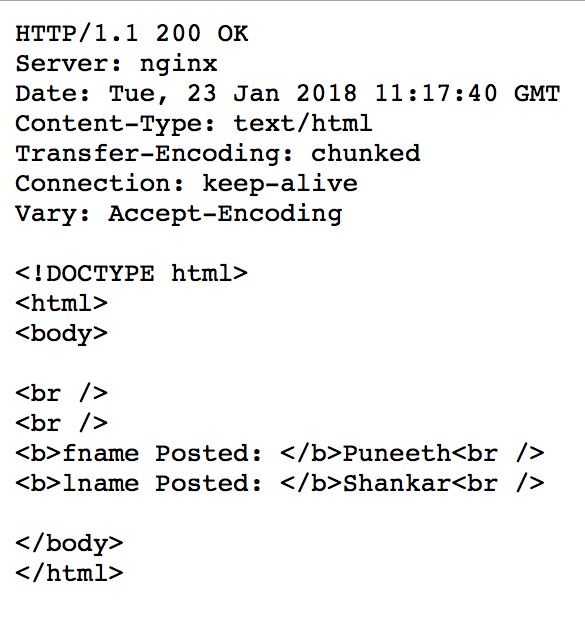
\includegraphics[width=0.5\textwidth]{webScience}
    %  \caption{Sample 'curl' with POST}
%\end{figure}
 
%}
\textbf{} All the raw HTML and the text contents can be found in the \textbf{Content} directory on github submission
  
\begin{lstlisting}[language=Python, caption=rawCode1.py]

import subprocess
from boilerpipe.extract import Extractor
import sys
import hashlib
reload(sys)
sys.setdefaultencoding('utf8')

linksDict = {}
linksFile = open('1000TwitterLinks.txt','r')
for link in linksFile:
	if(link == ''):
		pass
	else:
		try:
			curlCommand = 'curl ' + link
			hash_object = hashlib.md5(link)
			print(hash_object.hexdigest() + '.html')
			htmlFile = hash_object.hexdigest() + ':htmlFile'
			textFile = hash_object.hexdigest() + ':txt'
			f = open(htmlFile, "w")
			raw_html = subprocess.call(curlCommand, shell=True, stdout=f)
			extractor = Extractor(extractor='ArticleExtractor', url=link)
			with open(textFile, 'w') as the_file:
				the_file.write(str(extractor.getText()))
				linksDict[textFile] = link
				print str(extractor.getText())

		except KeyboardInterrupt:
			exit()		
		except:
			pass


with open('textURLFile', 'w') as file:
	for key,value in linksDict.items():
		file.write('%s:%s\n' % (key, value))	

\end{lstlisting}

The above code will save the Text File name and the URI in to \textbf{"textURLFile.txt"} file, as attached in github. 

\end{homeworkProblem}
\clearpage
\newpage

%----------------------------------------------------------------------------------------
%   PROBLEM 2
%----------------------------------------------------------------------------------------

\begin{homeworkProblem}
 
Choose a query term (e.g., "shadow") that is not a stop word (see week 5 slides) and not HTML markup from step 1 (e.g., "http") that matches at least 10 documents (hint: use "grep" on the processed
files).  If the term is present in more than 10 documents, choose any 10 from your list.\\

Compute TFIDF values for the term in each of the 10 documents and create a table with the TF, IDF, and TFIDF values, as well as the corresponding URIs.  The URIs will be ranked in decreasing order 
by TFIDF values.\\

 
 
%\problemAnswer{
 \textbf{SOLUTION}\\\\
 The solution for this problem is outlined by the following steps:
 
 \begin{enumerate}
   \item The program requires to run the 'GREP' command over all the text files obtained during Problem 1. 
  		        
	     \textbf{} 1. GREP will find the text \textbf{"goals"} on the processed files
  			\begin{verbatim}
			 	cmd = "grep -ci 'goals' * > grepOutput.txt"
				  subprocess.call(cmd, shell=True)	
				\end{verbatim}
 			The output of the above step would return filenames of the processed files whose hit count is more than 0\\
			
 	    \textbf{}  2. To calculate the terms to tabulate for every URI, the code determines TF ,IDF and TFIDF values
	    		 \begin{verbatim}
			  Term Frequency (TF) = 
			               Number of occurrences of the word / Total number of words
			  Inverse Document Frequency (IDF) = 
			     log2(total URIs in corpus/total processed files with term 'goals')
			  TF-IDF = TF * IDF
			 \end{verbatim}
 \end{enumerate}
 
\begin{lstlisting}[language=Python, caption=rawCode2.py]
import subprocess
import math

cmd = "grep -ci 'goals' * > grepOutput.txt"
subprocess.call(cmd, shell=True)
count = 0
matchCount = round(0,4)
corpusCount = round(0,4)
docsWithTerm = round(0,4)
idf = round(0,4)
tf = round(0,4)
tfidf = round(0,4)
totalWordsInFile = round(0,4)
num_words = 0
tfDict = {}

def countWordsInFile(fileName):
	global num_words
	with open(fileName, 'r') as f:
		for line in f:
			words = line.split()
			num_words += len(words)
	return num_words
	
linksFile = open('grepOutput.txt','r')
for line in linksFile:
	line = line.replace('\n', '')
	
	if(':txt' in line):
		matchCount = round(int(line[(line.rfind(':')+1):]),4)
		corpusCount = corpusCount + 1
		if(matchCount >= 1):
			line  = line[0:line.rfind(':')]
			totalWordsInFile = countWordsInFile(line)
			print ('line',line)
			print('Total Words :',totalWordsInFile)
			print ('matchCount',matchCount)
			docsWithTerm = docsWithTerm + 1
			tf = round((matchCount / totalWordsInFile),4)
			if(tf >= 0.0003):
				tfDict[line] = tf
			print('\n')
	else:
		continue	
 		
# idf = round((corpusCount / docsWithTerm),4)

idf = math.log(round((corpusCount / docsWithTerm),4)) / math.log(2)
tfidf = round((tf * idf),4) 

print('TFIDF    TF    IDF    	    URL')
print('-----    --    ---    	    ---')

data = dict()
with open('textURLFile','r') as raw_data:
    for item in raw_data:
        if ':txt' in item:
            key,value = item.split(':txt:', 1)
            data[key]=value
        else:
            pass
 
for key, value in tfDict.items(): 
	 key = key[0:key.rfind(':')]  
	 tfIdfValue = round((float(value) * idf),4)
	 tfValue = value
	 url = data[key]
	 print(str(tfIdfValue)+'   '+str(tfValue)+'   '+str(idf)+'   '+url)
	
\end{lstlisting} 
%}


\textbf{} The output of the code execution can be found in the \textbf{"P3_Output.txt"} 

\newpage
\begin{lstlisting}[caption=Extracted ratios] 

TFIDF    TF    IDF    	    URL
-----    ---   ---    	    ---
0.001   0.0003   3.3513315059   https://www.thescottishsun.co.uk/sport/football
/2216776/huddersfield-star-accidentally-flashes-xxxxx-to-millions-worldwide-on-
live-tv-during-premier-league-clash-with-bournemouth/

0.0013   0.0004   3.3513315059   https://www.chelseafc.com/news/latest-news
/2018/02/home-and-away--eidur-gudjohnsen.html

0.0017   0.0005   3.3513315059   http://www.independent.co.uk/sport/football/
premier-league/manchester-united-munich-air-disaster-wembley-sport-greatest
-ever-stories-a8195736.html

0.001   0.0003   3.3513315059   http://www.gulf-times.com/story/581358/Nepal
-plays-2-2-against-Lebanon-in-Asian-Football-

0.001   0.0003   3.3513315059   http://www.und.com/sports/m-baskbl/spec-rel/
021118aaa.html

0.001   0.0003   3.3513315059   https://pechalbata.com/super-vip-football-
predictions-2-02-2018/

0.001   0.0003   3.3513315059   https://www.birminghammail.co.uk/sport/football/
football-news/john-terry-villa-birmingham-city-14276580

0.001   0.0003   3.3513315059   https://www.mirror.co.uk/sport/football/
match-reports/electric-egyptian-mo-salah-just-12009750

0.0013   0.0004   3.3513315059   https://www.onefootdown.com/2018/2
/11/17000964/womens-lacrosse-notre-dame-loses-boston-college-maddie
-howe-nikki-ortega-irish-eagles-acc-sam-apuzzo

0.001   0.0003   3.3513315059   https://www.liverpoolecho.co.uk/sport/football/
football-news/jurgen-klopp-reveals-details-conversation-14276564

0.0044   0.0013   3.3513315059   https://www.coventrytelegraph.net/sport/football/
football-news/coventry-city-fc-player-ratings-14273283?service=responsive

0.0158   0.0047   3.3513315059   https://www.sportsmole.co.uk/football/wolves/news/
nuno-wolves-worthy-winners-against-qpr_318467.html

0.001   0.0003   3.3513315059   https://itunes.apple.com/us/app/soccer-
agent-football-manager/id1021569826?mt=8

0.001   0.0003   3.3513315059   https://www.youtube.com/watch?v=bKMZmEeqHQA&
feature=youtu.be

0.002   0.0006   3.3513315059   http://www.skysports.com/football/news/
11661/11245990/southampton-0-2-liverpool-mohamed-salah-roberto-firmino-
star-on-virgil-van-dijk-return

\end{lstlisting}
 
\end{homeworkProblem}
\clearpage
\newpage

%----------------------------------------------------------------------------------------
%   PROBLEM 3
%----------------------------------------------------------------------------------------

\begin{homeworkProblem}
Now rank the same 10 URIs from question 2, but this time  by their PageRank.  Use any of the free PR estimaters on the web,
Such as:
 \begin{verbatim}
http://pr.eyedomain.com/
http://www.prchecker.info/check_page_rank.php
http://www.seocentro.com/tools/search-engines/pagerank.html
http://www.checkpagerank.net/
\end{verbatim}
 

%\problemAnswer{

 \textbf{SOLUTION}\\
 
 \textbf{} The below Page Ranks are obtained manually from the below ranking site : \\
\begin{verbatim}
               http://www.checkpagerank.net/
\end{verbatim}

\begin{lstlisting}[caption=PageRank]
PageRank		URI
--------		---
0.5			https://www.thescottishsun.co.uk
0.7			https://www.chelseafc.com
0.9			http://www.independent.co.uk
0.7			http://www.gulf-times.com
0.5			http://www.und.com
0.4			https://pechalbata.com
0.7			https://www.birminghammail.co.uk
0.8			https://www.mirror.co.uk
0.5			https://www.onefootdown.com
0.6			https://www.liverpoolecho.co.uk
0.8			https://www.coventrytelegraph.net
0.5			https://www.sportsmole.co.uk
0.9			https://itunes.apple.com
1			https://www.youtube.com
0.7			http://www.skysports.com	
				
\end{lstlisting}
   
%}

\end{homeworkProblem}
\clearpage
\newpage

\bibliographystyle{plain}
\bibliography{A1bibFile}

\end{document}
